\subsection{The Lower Bound}
As mentioned previously in this chapter the lower bound is the number of twists required to solve the \rubik{} in the position which requires the most twists to solve. 
For now it is proven that the superflip position(see figure \ref{fig:superflip}), is the position which requires the most twists to be solved \cite{speedsolving.wiki}.
The shortest path from the superflip to the solved position is 20 twists \cite{rokicki09}.
This has been proven by trying every possible solutions with 19 twists or less. 
There has not been found a position that requires more than 20 twists, which makes the lower bound 20 twists.

\begin{figure}[ht]
	\centering
		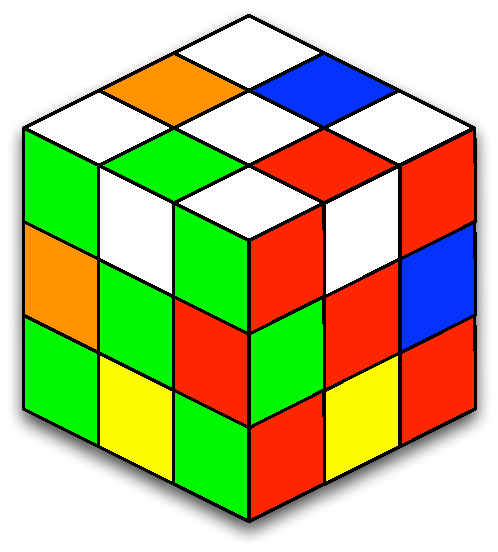
\includegraphics[scale = 0.7]{input/pics/superflip.pdf}
	\caption{\myCaption{The superflip: every edge is flipped. The optimal solution to this position is 20 twists.}}
	\label{fig:superflip}
\end{figure}



